\section{Background and Motivation}
\label{sec:example}

\PUNT{
We first demonstrate how learning addresses complexity, while even
advanced, adaptive controllers cannot.  We then show how control
theory handles system dynamics.  We conclude this section by
demonstrating what can go wrong when a controller incorporates a
learned model without proper tuning.
}
Many machine learning approaches estimate the most energy efficient
set of resources to allocate to an application.  These include
\emph{offline} techniques that build models using a training set and
then apply those models to new applications
\cite{Yi2003,LeeBrooks2006,CPR,ChenJohn2011,reddiHPCA2013,Paragon,PUPiL}.
Other approaches use \emph{online} techniques that construct models
dynamically as an application runs
\cite{Li2006,Flicker,ParallelismDial,Ponamarev,LeeBrooks}.  Finally,
\emph{hybrid} techniques combine offline modeling with online model
updates \cite{Zhang2012,packandcap,Winter2010,dubach2010,Koala,Cinder,
  wu2012inferred,LEO}.  

Machine learning is well suited to building
models of complicated systems like heterogeneous ARM big.LITTLE
systems.  These processors have two different core types including:
four big high-performance cores and four LITTLE energy efficient
cores.  The big cores support 19 clock speeds, while the LITTLE cores
support 14.

Control theory is a collection of mechanisms for maintaining required
behavior in dynamic systems \cite{Hellerstein2004a}. A subset of these
mechanisms---known as \emph{adaptive control} or \emph{self-tuning
  regulators}---are highly resilient to external effects that alter
behavior.  Adaptive controllers are thus especially useful in
webservers with fluctuating request rates
\cite{Horvarth,LuEtAl-2006a,SunDaiPan-2008a} and multimedia
applications with dynamically varying inputs
\cite{TCST,Agilos,grace2}.  Prior control solutions, however, are
always highly application dependent---with application-specific models
encoded in the controller's design---making a controller for video
playback unsuitable for controlling GPS navigation.  Some prior work
has generalized adaptive control design by exposing key parameters to
users so that the controller can be customized for a user's needs
\cite{ControlWare,POET}.  
This provides greater flexibility to the users but the controller can still fail to converge to the desired performance if there is mischaracterization in the relationship between resources and performance.  \PUNT{This limitation
  is why existing adaptive control approaches are built for specific
  classes of applications---specializing for the class accounts for
  common non-convexities of that class.}

\subsection{\emph{Learning} Complexity}
\PUNT{
\begin{figure*}
\centering
  \subfloat[]
  {
    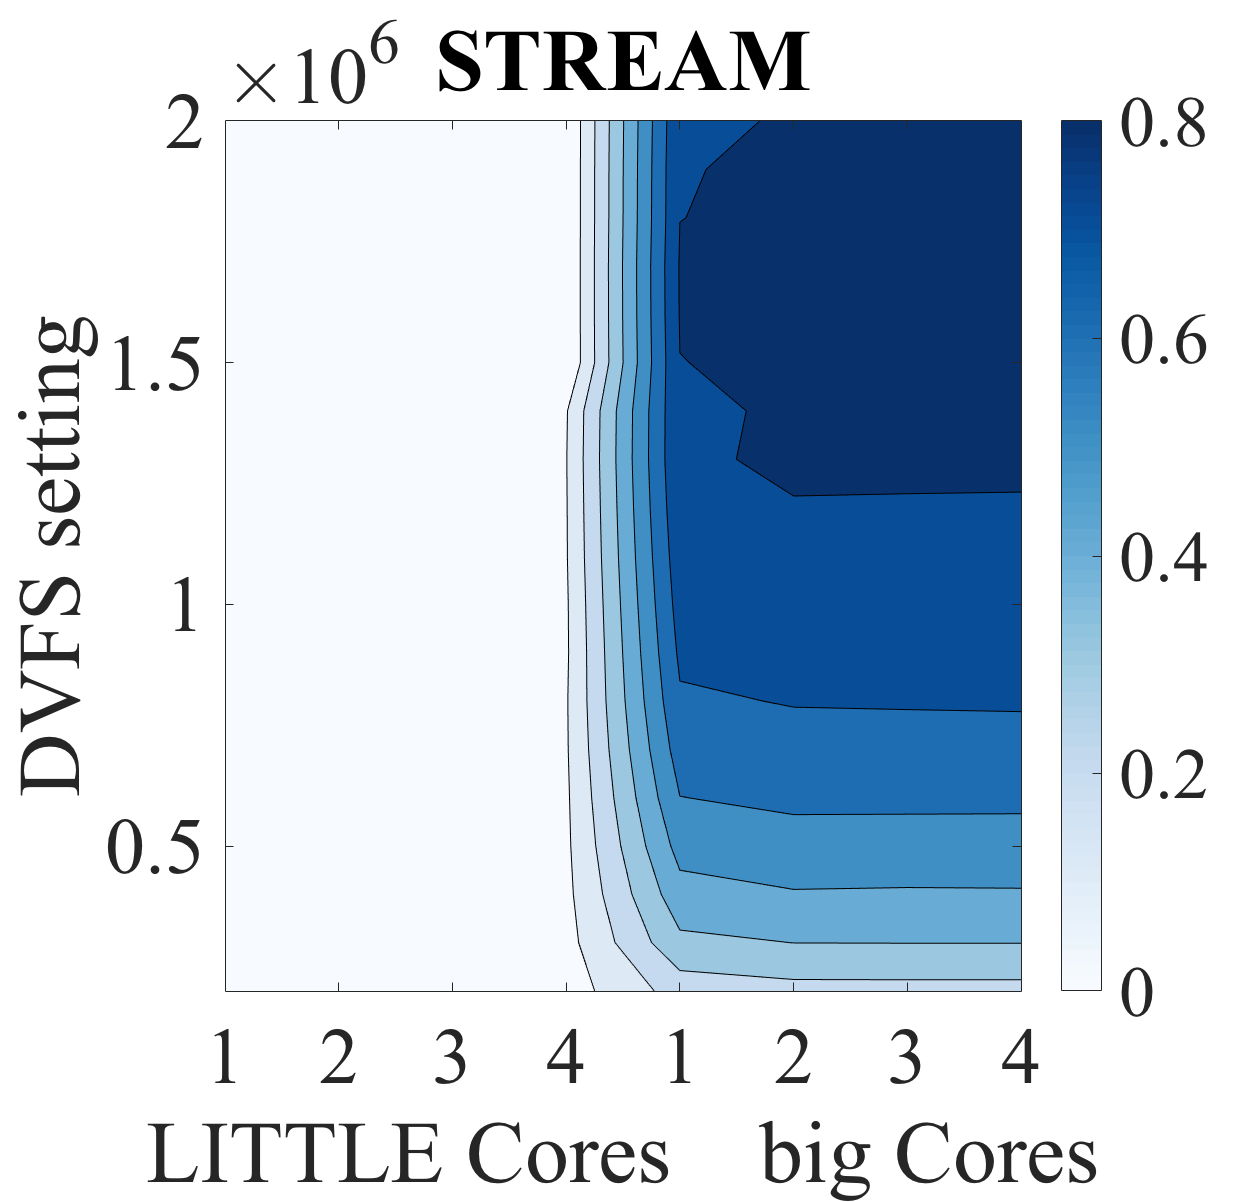
\includegraphics[width=.25\textwidth]{figures/STREAM-contour.png}
    \label{fig:STREAM_contour}
  }
  \subfloat[]
  {
    \begin{tikzpicture}
\begin{centering}

\definecolor{s1}{RGB}{228, 26, 28}
\definecolor{s2}{RGB}{55, 126, 184}
\definecolor{s3}{RGB}{77, 175, 74}
\definecolor{s4}{RGB}{152, 78, 163}
\definecolor{s5}{RGB}{255, 127, 0}

\begin{groupplot}[
    group style={
        group name=plots,
        group size=1 by 1,
        xlabels at=edge bottom,
        xticklabels at=edge bottom,
        vertical sep=5pt
    },
height=4.1cm,
width=0.45\columnwidth,
xmajorgrids,
ymajorgrids,
grid style={dashed},
xmax=20,
yticklabel pos=left,
enlargelimits=false,
tick align = outside,
tick style={white},
xticklabel shift={-5pt},
yticklabel shift={-5pt},
ylabel shift={-2pt},
ylabel style={align=center},
unbounded coords=jump,
]

\nextgroupplot[ylabel={\scriptsize Performance (Normalized)}, % Performance
xlabel={\footnotesize Iteration},
ymin=0,
ymax=1.5,
ytick={0.0,0.5,1.0,1.5},
yticklabels={,0.5,1.0,1.5},
legend entries={{\scriptsize $\mathsf{Performance Requirement}$},{\scriptsize $\mathsf{Learning}$},{\scriptsize $\mathsf{Adaptive Control}$},},
legend style={fill=none,draw=none,at={(0.5,1.4)},anchor=north,legend columns=1,line width=3pt},
]

\addplot[thick, solid, black] coordinates {(0,1) (20,1)};
\addplot[thick, solid, color=s4] table[x index=0,y index=1,col sep=space] {img/complexity-example-leo.txt};
\addplot[thick, solid, color=s5] table[x index=0,y index=1,col sep=space] {img/complexity-example-poet.txt};
\end{groupplot}
\end{centering}
\end{tikzpicture}
    \label{fig:STREAM_timeline}
  }
  \subfloat[]
  {
    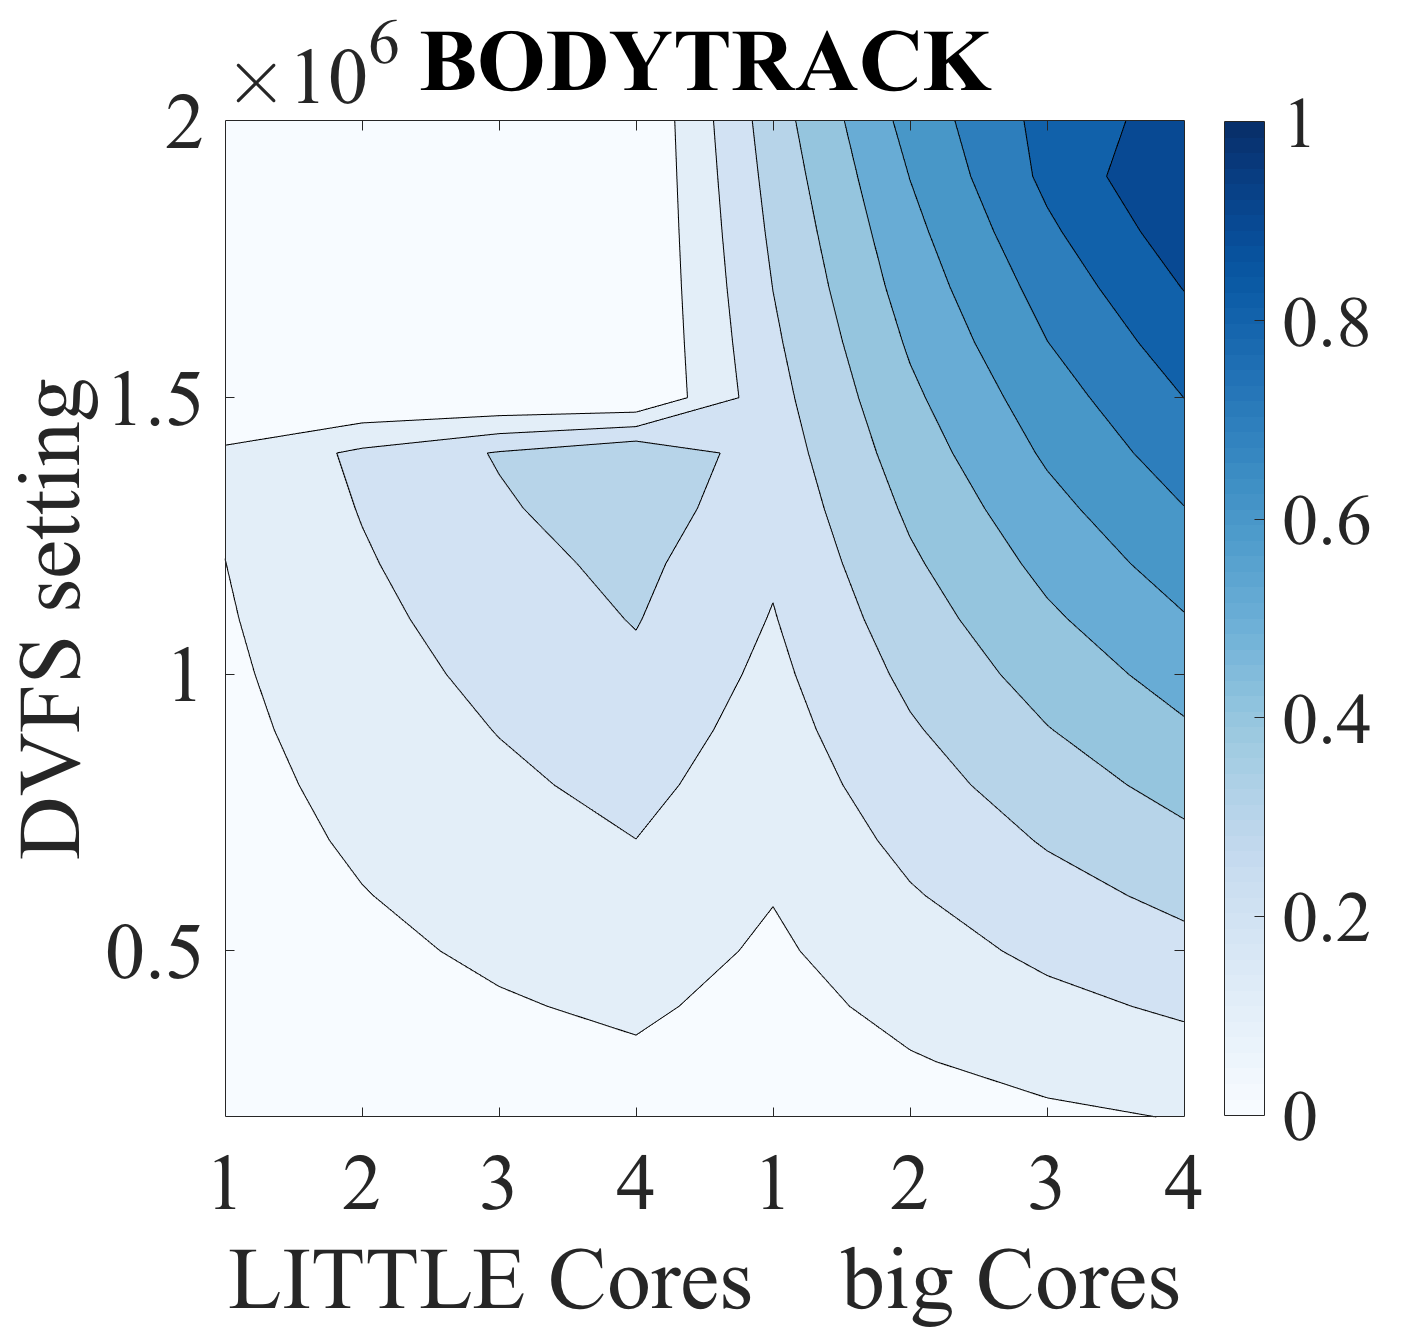
\includegraphics[width=.25\textwidth]{figures/BODYTRACK-contour.png}
    \label{fig:BODYTRACK_contour}
  }
  \subfloat[]
  {
    \begin{tikzpicture}
\begin{centering}

\definecolor{s1}{RGB}{228, 26, 28}
\definecolor{s2}{RGB}{55, 126, 184}
\definecolor{s3}{RGB}{77, 175, 74}
\definecolor{s4}{RGB}{152, 78, 163}
\definecolor{s5}{RGB}{255, 127, 0}

\begin{groupplot}[
    group style={
        group name=plots,
        group size=1 by 1,
        xlabels at=edge bottom,
        xticklabels at=edge bottom,
        vertical sep=5pt
    },
height=3.5cm,
width=0.45\columnwidth,
xmajorgrids,
ymajorgrids,
grid style={dashed},
xmin=0,
xmax=20,
yticklabel pos=left,
enlargelimits=false,
tick align = outside,
tick style={white},
xticklabel shift={-5pt},
yticklabel shift={-5pt},
ylabel shift={-2pt},
ylabel style={align=center},
unbounded coords=jump,
]

\nextgroupplot[ylabel={\scriptsize Performance (Normalized)}, % Performance
%xtick={0,500,1000,1500,2000,2500,3000,3500,4000,4500},
ytick={0.0,0.5,1.0,1.5,2.0},
yticklabels={,0.5,1.0,1.5,2.0},
xtick={90,95,100,105,110},
xticklabels={90,95,100,105,110},
%yticklabel style={font=\footnotesize},
xlabel={\footnotesize frame},
xmin=90,
xmax=110,
ymin=0,
ymax=1.5,
legend entries={{\scriptsize $\mathsf{Performance Requirement}$},{\scriptsize $\mathsf{Learning}$},{\scriptsize $\mathsf{Adaptive Control}$}},
legend style={fill=none,draw=none,at={(0.5,1.65)},anchor=north,legend columns=1,
line width=5pt},
]

\addplot[thick, solid, black] coordinates {(0,1) (399,1)};
\addplot[thick, solid, color=s4, mark=o] table[x index=0,y index=1,col sep=space] {img/dynamics-example-leo.txt};
\addplot[thick, solid, color=s5, mark=square] table[x index=0,y index=1,col sep=space] {img/dynamics-example-poet.txt};
\addplot[thick, dashed, black] coordinates {(99,0) (99,1.5)};
%\addplot[thick, dashed, black] coordinates {(130,0) (130, 2)};
\end{groupplot}
\end{centering}

\end{tikzpicture}

    \label{fig:BODYTRACK_timeline}    
  }
  \caption{\small \bf (a) Performance for \texttt{STREAM} as a
    function of configuration.  (b) Managing \texttt{STREAM}'s
    performance: \emph{Learning} navigates the complicated
    configuration space, but \emph{control}'s simple model leads to
    oscillation.  (c) Performance for \texttt{bodytrack} as a function
    of configuration. (d) Managing \texttt{bodytrack}'s performance
    when another application starts: \emph{Adaptive Control} detects
    the change and adjusts, but \emph{Learning} has no mechanism to
    handle these dynamics. }
  \label{fig:learning-models1}
\end{figure*}
}

\begin{figure}
\centering
  \subfloat[]
  {
    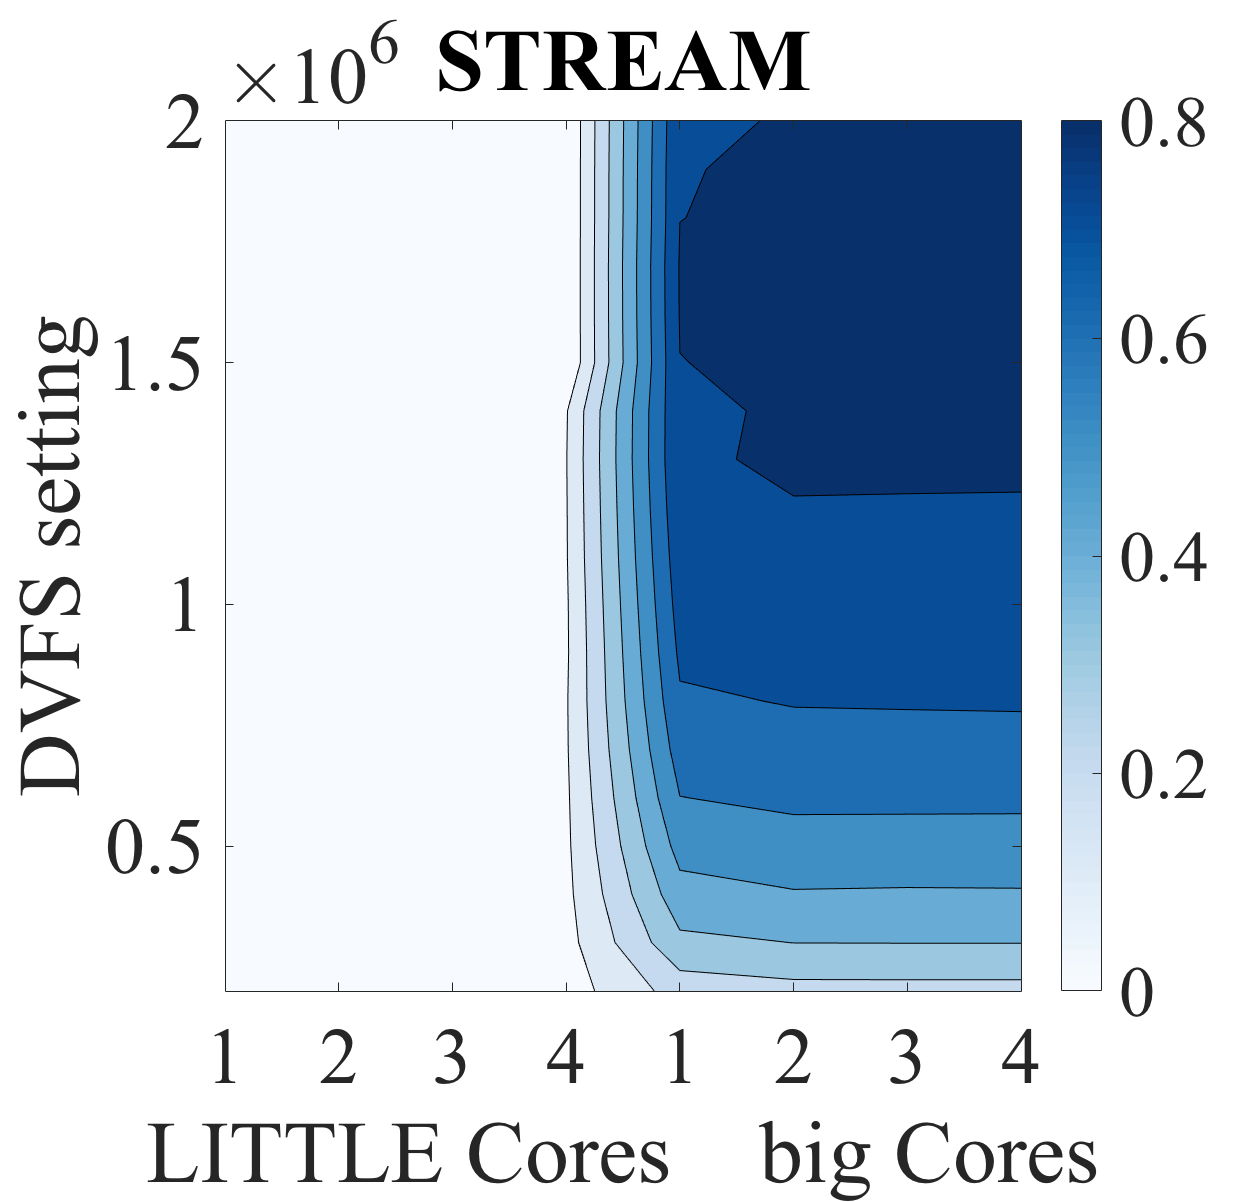
\includegraphics[width=.25\textwidth]{figures/STREAM-contour.png}
    \label{fig:STREAM_contour}
  }
  \subfloat[]
  {
    \begin{tikzpicture}
\begin{centering}

\definecolor{s1}{RGB}{228, 26, 28}
\definecolor{s2}{RGB}{55, 126, 184}
\definecolor{s3}{RGB}{77, 175, 74}
\definecolor{s4}{RGB}{152, 78, 163}
\definecolor{s5}{RGB}{255, 127, 0}

\begin{groupplot}[
    group style={
        group name=plots,
        group size=1 by 1,
        xlabels at=edge bottom,
        xticklabels at=edge bottom,
        vertical sep=5pt
    },
height=4.1cm,
width=0.45\columnwidth,
xmajorgrids,
ymajorgrids,
grid style={dashed},
xmax=20,
yticklabel pos=left,
enlargelimits=false,
tick align = outside,
tick style={white},
xticklabel shift={-5pt},
yticklabel shift={-5pt},
ylabel shift={-2pt},
ylabel style={align=center},
unbounded coords=jump,
]

\nextgroupplot[ylabel={\scriptsize Performance (Normalized)}, % Performance
xlabel={\footnotesize Iteration},
ymin=0,
ymax=1.5,
ytick={0.0,0.5,1.0,1.5},
yticklabels={,0.5,1.0,1.5},
legend entries={{\scriptsize $\mathsf{Performance Requirement}$},{\scriptsize $\mathsf{Learning}$},{\scriptsize $\mathsf{Adaptive Control}$},},
legend style={fill=none,draw=none,at={(0.5,1.4)},anchor=north,legend columns=1,line width=3pt},
]

\addplot[thick, solid, black] coordinates {(0,1) (20,1)};
\addplot[thick, solid, color=s4] table[x index=0,y index=1,col sep=space] {img/complexity-example-leo.txt};
\addplot[thick, solid, color=s5] table[x index=0,y index=1,col sep=space] {img/complexity-example-poet.txt};
\end{groupplot}
\end{centering}
\end{tikzpicture}
    \label{fig:STREAM_timeline}
  }
  \caption{\small \bf (a) Performance for \texttt{STREAM} as a
    function of configuration.  (b) Managing \texttt{STREAM}'s
    performance: \emph{Learning} navigates the complicated
    configuration space, but \emph{control} leads to oscillation.}
  \label{fig:learning-models1}
\end{figure}

We demonstrate how well learning manages complexity by considering a
performance requirement for \texttt{STREAM} on our ARM big.LITTLE
processor, which has the complicated configuration space illustrated
in \figref{fig:STREAM_contour}.  This memory-bound application has
complicated behavior: due to memory pressure, the LITTLE cores' memory
hierarchy cannot deliver the required performance.  The big cores'
more powerful memory system delivers much greater performance, but the
peak occurs with 3 big cores.  Furthermore, at low clockspeeds, these
3 big cores cannot saturate the memory bandwidth, while at high
clockspeeds the performance drops as the processor overheats and
triggers thermal management.  For \texttt{STREAM}, the peak speed
occurs with 3 big cores at 1.2 GHz, and it is not efficient to spend
any time on the LITTLE cores.  \texttt{STREAM}, however, does not have
distinct phases, so once a resource allocator finds the most energy
efficient configuration, it simply needs to maintain it.  \TODO{We
  should change the levels in the contour so there is a clear maximum
  at 3 cores and a middle clock speed.}

We use both a hierarchical Bayesian \emph{learning} model \cite{LEO}
and an \emph{adaptive control} system \cite{POET} to meet a
performance requirement with minimal energy.  The \emph{learning}
approach estimates the application's performance and power for all
configurations and then uses the lowest power configuration that
delivers the required performance.  The \emph{adaptive controller}
begins with a generic model of power/performance tradeoffs.  As the
controller runs, it continually measures performance and adjusts both
allocated resources and its internal models to tailor its response to
the current application.  While many controllers use linear models,
this adaptive controller dynamically adjusts to non-linearities with a
series of linear approximations; however, the adaptive controller is
sensitive to local maxima, which can cause oscillations and prevent
the controller from meeting the requirement.

\figref{STREAM_timeline} shows 20 iterations of \texttt{STREAM}.  The
x-axis shows iteration number and the y-axis shows performance
normalized to the requirement.  The learning approach achieves the
goal, but the adaptive controller oscillates wildly around it,
sometimes not achieving the goal and sometimes delivering performance
that is too high (and wastes energy).  The oscillations occur because
the controller's adaptive mechanisms cannot handle the non-convexity
in STREAM's behavior, a known limitation of adaptive control systems
\cite{ControlWare,POET,ICSE2014}.  Hence, the \emph{learner}'s ability
to handle complex behavior is crucial for reliable performance in this
example.

% This result may be somewhat counter-intuitive.  The problem is that
% the controller cannot handle \texttt{STREAM}'s complexity.  One way to
% address this problem would be to build a custom controller just for
% this application, but that controller would not be useful for other
% applications.  In contrast, the learner can find the local maxima in
% the configuration space, and as this application has no phase changes
% or other dynamics, the one configuration that the learner finds is
% suitable for the entire application.

\subsection{\emph{Controlling} Dynamics}

\PUNT{
\begin{figure*}
\centering
  \subfloat[]
  {
    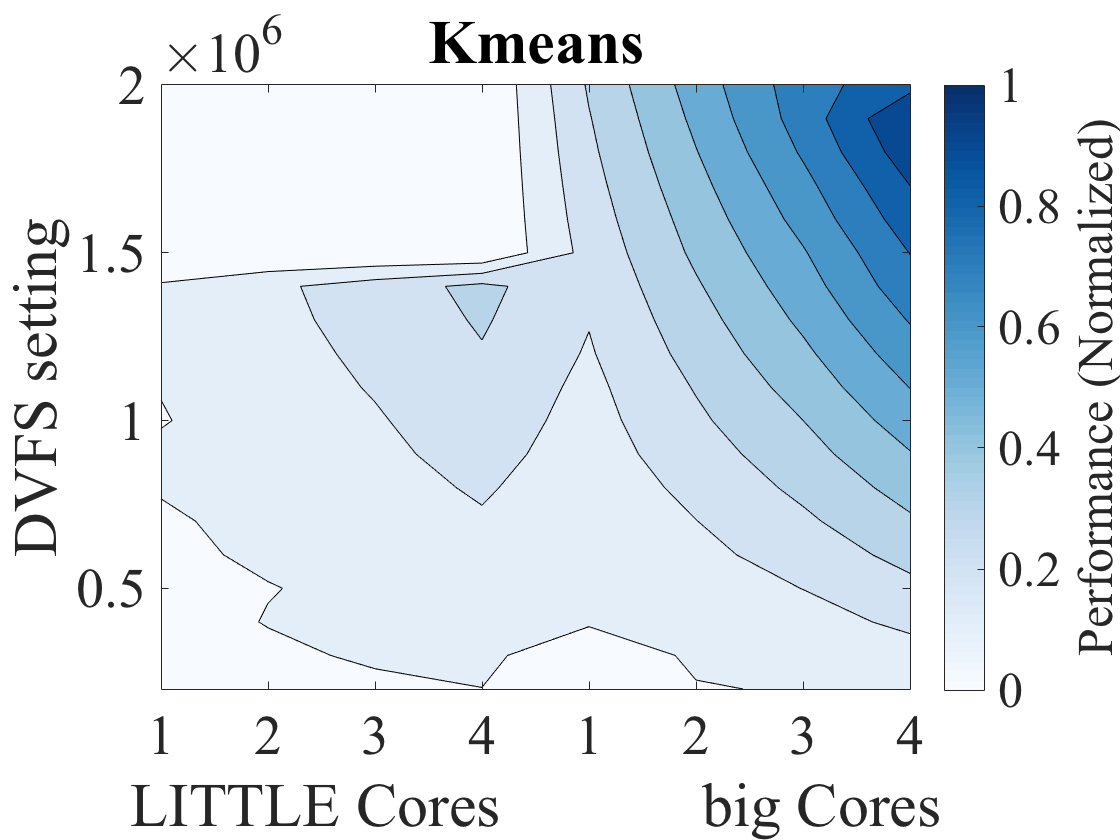
\includegraphics[width=.25\textwidth]{figs/kmeans.png}
    \label{fig:kmeans_contour}
  }
  \subfloat[]
  {
    \begin{tikzpicture}
\begin{centering}

\definecolor{s1}{RGB}{228, 26, 28}
\definecolor{s2}{RGB}{55, 126, 184}
\definecolor{s3}{RGB}{77, 175, 74}
\definecolor{s4}{RGB}{152, 78, 163}
\definecolor{s5}{RGB}{255, 127, 0}

\begin{groupplot}[
    group style={
        group name=plots,
        group size=1 by 1,
        xlabels at=edge bottom,
        xticklabels at=edge bottom,
        vertical sep=5pt
    },
height=4cm,
width=1.3\columnwidth,
xmajorgrids,
ymajorgrids,
grid style={dashed},
xmin=0,
xmax=20,
yticklabel pos=left,
enlargelimits=false,
tick align = outside,
tick style={white},
xticklabel shift={-5pt},
yticklabel shift={-5pt},
ylabel shift={-2pt},
ylabel style={align=center},
unbounded coords=jump,
]

\nextgroupplot[ylabel={\footnotesize Performance \\ (Normalized)}, % Performance
%xtick={0,500,1000,1500,2000,2500,3000,3500,4000,4500},
ytick={0.0,0.5,1.0,1.5,2.0},
yticklabels={,0.5,1.0,1.5,2.0},
%xtick={0,30,60,120,160,200,240,280,320,480},
%xticklabels={,0,30,60,120,160,200,240,280,320,480},
%yticklabel style={font=\footnotesize},
xlabel={\footnotesize time (in sec)},
ymin=0,
ymax=1.5,
legend entries={,{$\mathsf{Learning}$},{$\mathsf{Control}$}},
legend style={draw=none,at={(0.5,1.3)},anchor=north,legend columns=4,
line width=5pt},
]

\addplot[thick, dashed, black] coordinates {(10,0) (10,1.5)};
\addplot[thick, solid, color=s4] table[x index=0,y index=1,col sep=tab] {img/image_text/kmeans-example.txt};
\addplot[thick, solid, color=s5] table[x index=0,y index=2,col sep=tab] {img/image_text/kmeans-example.txt};
%\addplot[thick, dashed, black] coordinates {(130,0) (130, 2)};
\end{groupplot}
\end{centering}

\end{tikzpicture}

    \label{fig:kmeans_timeline}    
  }
  \caption{\small \bf (a) Performance for \texttt{kmeans} as a function of
    configuration.  (b) Managing \texttt{kmeans}' performance when
    another application starts: \emph{Control} detects the change and
    adapts, but \emph{learning} has no mechanism to handle these
    dynamics.}
  \label{fig:learning-models2}
\end{figure*}
} 


\begin{figure}
\centering
  \subfloat[]
  {
    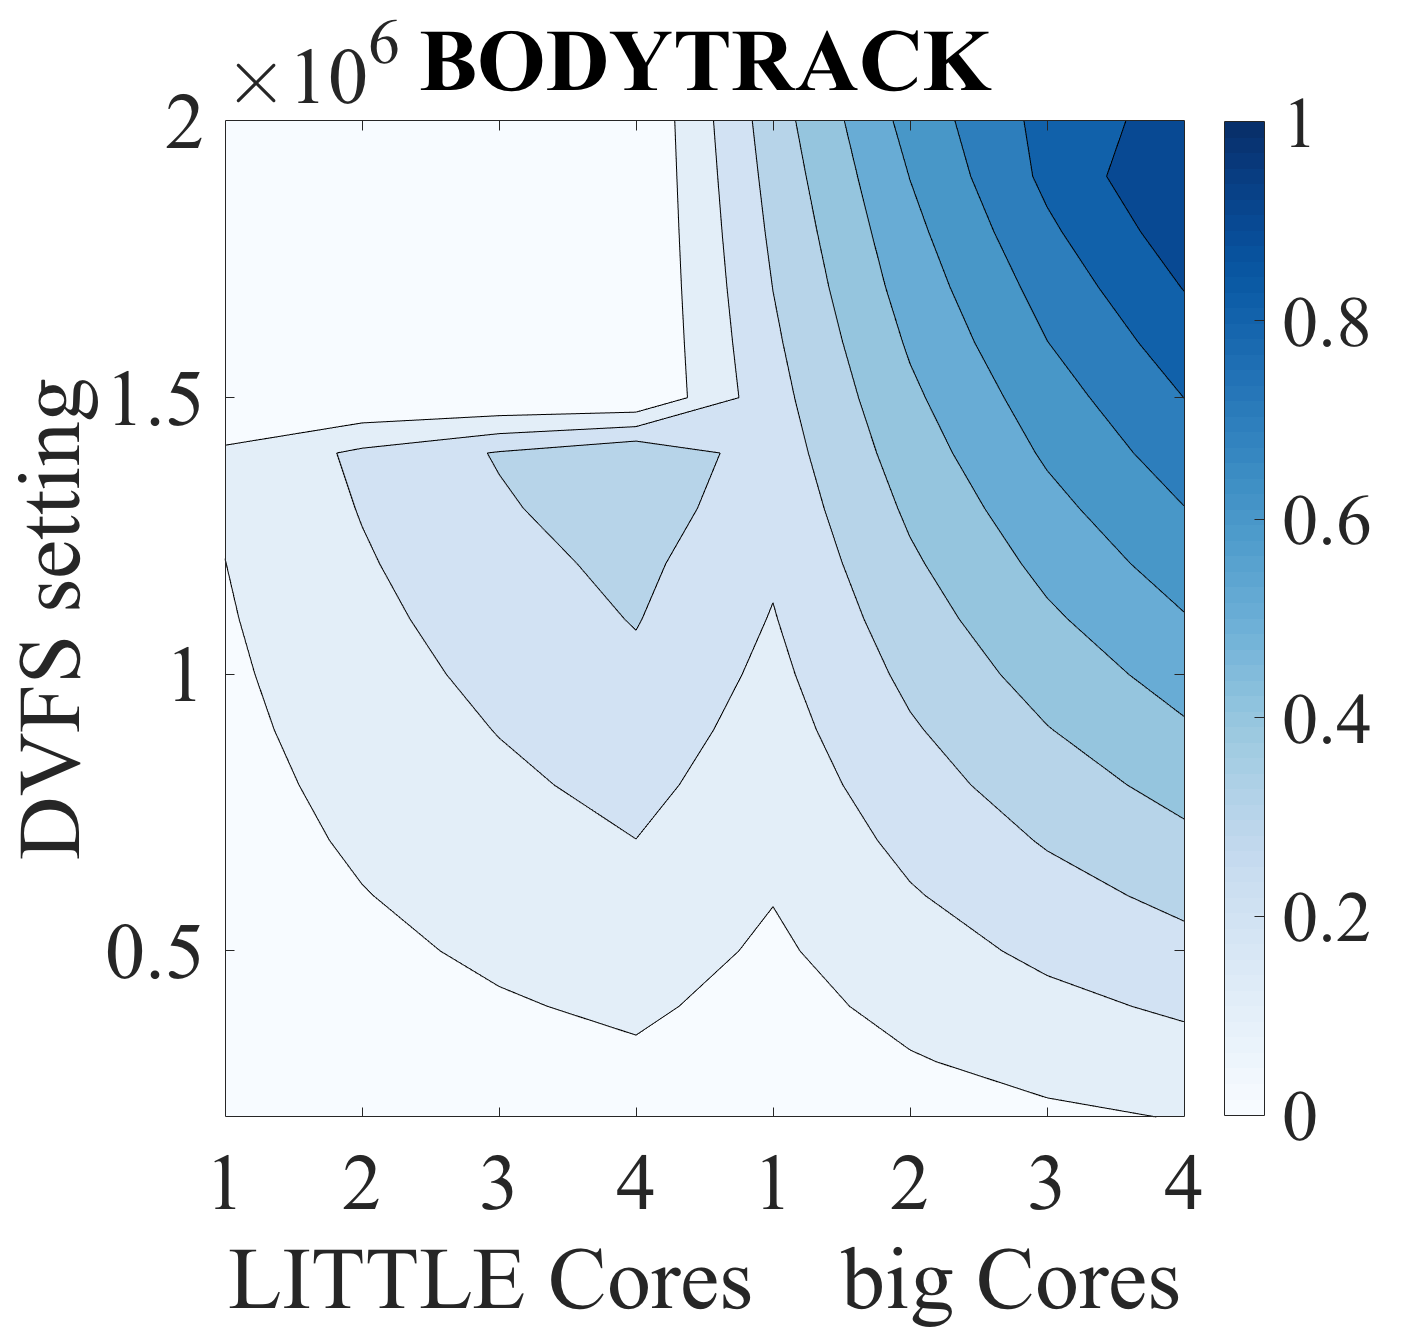
\includegraphics[width=.25\textwidth]{figures/BODYTRACK-contour.png}
    \label{fig:BODYTRACK_contour}
  }
  \subfloat[]
  {
    \begin{tikzpicture}
\begin{centering}

\definecolor{s1}{RGB}{228, 26, 28}
\definecolor{s2}{RGB}{55, 126, 184}
\definecolor{s3}{RGB}{77, 175, 74}
\definecolor{s4}{RGB}{152, 78, 163}
\definecolor{s5}{RGB}{255, 127, 0}

\begin{groupplot}[
    group style={
        group name=plots,
        group size=1 by 1,
        xlabels at=edge bottom,
        xticklabels at=edge bottom,
        vertical sep=5pt
    },
height=3.5cm,
width=0.45\columnwidth,
xmajorgrids,
ymajorgrids,
grid style={dashed},
xmin=0,
xmax=20,
yticklabel pos=left,
enlargelimits=false,
tick align = outside,
tick style={white},
xticklabel shift={-5pt},
yticklabel shift={-5pt},
ylabel shift={-2pt},
ylabel style={align=center},
unbounded coords=jump,
]

\nextgroupplot[ylabel={\scriptsize Performance (Normalized)}, % Performance
%xtick={0,500,1000,1500,2000,2500,3000,3500,4000,4500},
ytick={0.0,0.5,1.0,1.5,2.0},
yticklabels={,0.5,1.0,1.5,2.0},
xtick={90,95,100,105,110},
xticklabels={90,95,100,105,110},
%yticklabel style={font=\footnotesize},
xlabel={\footnotesize frame},
xmin=90,
xmax=110,
ymin=0,
ymax=1.5,
legend entries={{\scriptsize $\mathsf{Performance Requirement}$},{\scriptsize $\mathsf{Learning}$},{\scriptsize $\mathsf{Adaptive Control}$}},
legend style={fill=none,draw=none,at={(0.5,1.65)},anchor=north,legend columns=1,
line width=5pt},
]

\addplot[thick, solid, black] coordinates {(0,1) (399,1)};
\addplot[thick, solid, color=s4, mark=o] table[x index=0,y index=1,col sep=space] {img/dynamics-example-leo.txt};
\addplot[thick, solid, color=s5, mark=square] table[x index=0,y index=1,col sep=space] {img/dynamics-example-poet.txt};
\addplot[thick, dashed, black] coordinates {(99,0) (99,1.5)};
%\addplot[thick, dashed, black] coordinates {(130,0) (130, 2)};
\end{groupplot}
\end{centering}

\end{tikzpicture}

    \label{fig:BODYTRACK_timeline}    
  }
  \caption{\small \bf (a) Performance for \texttt{bodytrack} as a
    function of configuration. (b) Managing \texttt{bodytrack}'s
    performance when another application starts: \emph{Adaptive
      Control} detects the change and adjusts, but \emph{Learning} has
    no mechanism to handle these dynamics. }
  \label{fig:control}
\end{figure}


We now consider a dynamic environment.  We begin with
\texttt{bodytrack} as the only application running on the system.
Halfway through its execution, we launch a second
application---\texttt{STREAM}---on a single big core, dynamically
altering resource availability. \texttt{bodytrack}'s behavior is
simpler than \texttt{STREAM} as shown in
\figref{fig:BODYTRACK_contour}; it achieves its best performance on 4
big cores at the maximum clockspeed.  The challenge of allocating
resources for this application is determining how much work to do on
the LITTLE cores (to conserve energy) while still meeting the
performance requirements.  The relationship between LITTLE and big
core performance is non-linear. 

\figref{bodytrack_timeline} shows the results of this experiment.  The
vertical dashed line---at frame 99---represents when the second
application begins.  The figure clearly shows the benefits of the
adaptive control system in this dynamic scenario.  When the second
application starts, the controller detects the change in
\texttt{bodytrack}'s performance and then changes resource allocation
(increasing clockspeed and moving bodytrack from 4 to 3 big cores).
The controller is not aware of the second application, rather it
observes \texttt{bodytrack}'s performance drop at frame 99 and
immediately restores performance in the next frame. The learning
system however, does not have any inherent mechanism to measure the
change or adapt to the altered performance.  While we could
theoretically add feedback to the learner and re-estimate the
configuration space whenever the environment changes, doing so is
impractical due to high overhead\cite{pargon,LEO}.


\subsection{Challenges of Parameter-free Control}
The learner illustrated above is parameter-free; \ie{} it has no
user-specifed parameters, but estimates all values from measurements.
The controller, in contrast, requires some user-specified parameters.
\SYSTEM{}'s goal is to provide a parameter-free approach that provides
the same formal guarantees as a controller with user-specified
parameters.

Perhaps the most essential parameter for a control system is the
\emph{pole} of its characteristic equation.  Control engineers tune
the pole to trade control response time for noise sensitivity.
Following standard control design, the pole is tuned based on a known
model.  This model may be an abstraction of the full system, but it is
considered to be ``ground truth'' \cite{Hellerstein2004a}. In a
computing system ground truth means that all possible configurations
the controller might select have been directly measured.  \SYSTEM{},
however, must tune the pole based on an estimated model, which may
have noise and/or errors.


\begin{figure}
\centering
\begin{tikzpicture}
\begin{centering}

\definecolor{s1}{RGB}{228, 26, 28}
\definecolor{s2}{RGB}{55, 126, 184}
\definecolor{s3}{RGB}{77, 175, 74}
\definecolor{s4}{RGB}{152, 78, 163}
\definecolor{s5}{RGB}{255, 127, 0}

\begin{groupplot}[
    group style={
        group name=plots,
        group size=1 by 1,
        xlabels at=edge bottom,
        xticklabels at=edge bottom,
        vertical sep=5pt
    },
height=4.1cm,
width=0.45\columnwidth,
xmajorgrids,
ymajorgrids,
grid style={dashed},
xmin=0,
xmax=20,
yticklabel pos=left,
enlargelimits=false,
tick align = outside,
tick style={white},
xticklabel shift={-5pt},
yticklabel shift={-5pt},
ylabel shift={-2pt},
ylabel style={align=center},
unbounded coords=jump,
]

\nextgroupplot[ylabel={\scriptsize Performance (Normalized)}, % Performance
%xtick={0,500,1000,1500,2000,2500,3000,3500,4000,4500},
ytick={0.0,0.5,1.0,1.5,2.0},
yticklabels={,0.5,1.0,1.5,2.0},
xtick={90,95,100,105,110},
xticklabels={90,95,100,105,110},
%yticklabel style={font=\footnotesize},
xlabel={\footnotesize frame},
xmin=90,
xmax=110,
ymin=0,
ymax=1.5,
legend entries={{\scriptsize $\mathsf{Performance Requirement}$},{\scriptsize $\mathsf{Adaptive Control}$},{\scriptsize $\mathsf{Learning \& Control}$}},
legend style={fill=none,draw=none,at={(0.5,1.3)},anchor=north,legend columns=1,
line width=5pt},
]

\addplot[thick, solid, black] coordinates {(0,1) (399,1)};
\addplot[thick, solid, color=s5] table[x index=0,y index=1,col sep=space] {img/dynamics-example-poet.txt};
\addplot[thick, solid, color=s3] table[x index=0,y index=1,col sep=space] {img/dynamics-example-leopoetnp.txt};
\addplot[thick, dashed, black] coordinates {(99,0) (99,1.5)};
%\addplot[thick, dashed, black] coordinates {(130,0) (130, 2)};
\end{groupplot}
\end{centering}

\end{tikzpicture}

\caption{\small \bf Comparison of existing adaptive control and a
  naive combination of control and learning.}
\label{fig:not-simple}
\end{figure}

To demonstrate the importance of the pole in the presence of a learned
model, we again show control of \texttt{bodytrack}, this time using
the adaptive control system from the previous subsection with a model
produced by the learner from the first subsection.  We compare the
control system with a carefully tuned pole to the same system using
the default pole provided by the controller developers---recall that
the pole is typically a user-specified parameter.  

\figref{fig:not-simple} shows the results.  The system with the
carefully tuned pole converges because the pole accounts for the error
in the learned model.  The system with the default pole, however
oscillates around the performance target, resulting in a number of
missed deadlines.  In addition, the frames that exceed the desired
performance waste energy because they spend much more time on the big,
inefficient cores than necessary.

The next section describes \SYSTEM{}'s approach to combining learning
and control that abstracts the controller's key parameters, so they
can be learned while the system runs.  Rather than have a user
carefully tune the pole, \SYSTEM{} incorporates the learner's
confidence interval and estimated variance to compute a pole that
provides proabilistic convergence guarantees.  


